\documentclass[%
12pt, %
final, % 
oneside, % 
onecolumn, %  
centertags]{article} % относится к классу article и размер шрифта 12 пунктовб, {article: статья, report: отчеты и диссертации, book: книга, letter: письмо}

% \usepackage{fontspec}
 
% \setmainfont{Times New Roman}

% \documentclass[a4paper, 12pt]{report}

\topmargin= -30pt % насколько сверху будет страница
\textheight= 650pt


\usepackage[utf8]{inputenc} % задает кодировку, utf-8 кодировка, включающая в себя знаки почти всех языков мира
\usepackage[english]{babel} % подключает необходимые языки, основным языком является английский

\selectlanguage{english} % настройки будут на английском, но писать будет на русском

\usepackage{euscript}
\usepackage{supertabular}

\renewcommand{\baselinestretch}{1.0} 

\usepackage[colorlinks=true,linkcolor=blue,unicode=true,urlcolor = blue]{hyperref} %hypered
\usepackage[pdftex]{graphicx} % для графики

\usepackage{amsthm, amssymb, amsmath, amsfonts} % математический пакет, математические шрифты
\usepackage{textcomp}
\usepackage[noend]{algorithmic}
\usepackage[ruled]{algorithm}
\usepackage{lipsum}
\usepackage{indentfirst}
\usepackage{babel}
\usepackage{pgfplots}
\usepackage{setspace}
\usepackage{xcolor}
\usepackage{hyperref}
\usepackage{subfigure}

\setcounter{secnumdepth}{5}
\setcounter{tocdepth}{5}
\newcommand\simpleparagraph[1]{%
  \stepcounter{paragraph}\paragraph*{\theparagraph\quad{}#1}}
\usepackage{listings}
% \usepackage{xcolor}
%\usepackage{minted}

\lstset { %
     language=C++,
     backgroundcolor=\color{black!5}, % set backgroundcolor
     basicstyle=\footnotesize,% basic font setting
}


\linespread{1.0} 
\setlength{\parindent}{2.4em}
\setlength{\parskip}{0.1em}

\pgfplotsset{compat=1.9}
\pgfplotsset{model/.style = {blue, samples = 100}} 
\pgfplotsset{experiment/.style = {red}}

\theoremstyle{plain}
\binoppenalty=10000

\newtheorem{theorem}{Theorem}[section] % theorem

\theoremstyle{definition}
% \newtheorem{definition}{Определение}[subsection]
\newtheorem{definition}{Definition}[subsection]

\theoremstyle{remark}
% \newtheorem{remark}{Замечание}[section]

% \newtheorem{corollary}{Следствие}

% \newtheorem{proposition}{Proposition}

% \newtheorem{example}{Пример}

% \newtheorem{lemma}{Лемма}[section]

\renewcommand*{\proofname}{Proof}

\graphicspath{ {./images/} }


% \usepackage{amsmath,amsfonts,amssymb, setspace}  % Разнообразные математические команды и значки
% \usepackage{indentfirst}     % Отступ в первом абзаце

% \pagestyle{empty}
\usepackage[left=2.5cm, right=1.5cm, top=2.5cm, bottom=2.5cm]{geometry}
\usepackage[medium]{titlesec}
\usepackage{graphicx}
% \graphicspath{ {./images/} }

\begin{document}

	\begin{titlepage} 
		\begin{center}
		\textbf{}\\[2.0cm]
		\LARGE FEDERAL STATE AUTONOMOUS EDUCATIONAL INSTITUTION OF HIGHER EDUCATION \\[0.5cm]
		\Large ITMO UNIVERSITY \\[3cm]
		\LARGE Report\\
		\Large MPI. Assignments $10-11$ \\
		\Large Parallel algorithms for the analysis and synthesis of data \\[4cm]


		\begin{flushright}
		Performed by\\
		Aleksandr Shirokov\\
		J4133c\\
		Accepted by\\
		Petr Andriushchenko

		Deadline: 21.12.21
		\end{flushright}

		\vfill 

		{\Large {St. Petersburg}} \par
		{\Large {2021}}
		\end{center} 
	\end{titlepage}

\tableofcontents
\newpage


\section{Assignments}

\subsection{Assignment 10. MPI. Sending and receiving messages without blocking. Ring exchange using non-blocking operations.}

\subsubsection{Formulation of the problem}

Complete the program \textsc{Assignment10.c.} Compile and run it.

Study the code carefully and explain how it works.

\subsubsection{Example of launch parameters and output. Detailed description of solution}

Code for \textbf{assignment 10} is \href{https:\//github.com/aptmess/parallel_algorithms/blob/master/HT/hw_mpi/Assignment10.c}{here}.

Compilation example: \textsc{mpic++ -o ./cpf/10.o Assignment10.c}

Launch example: \textsc{mpirun --oversubscribe -np 10 ./cpf/10.o}

\begin{center}
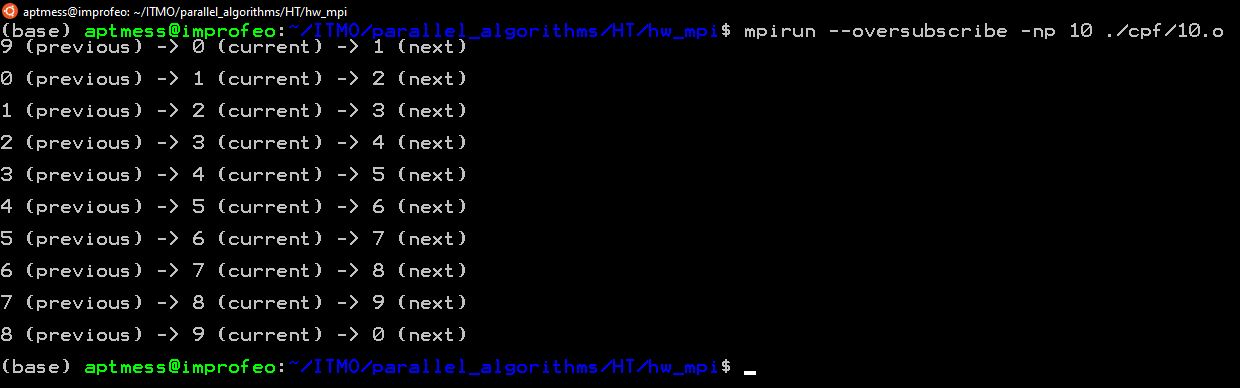
\includegraphics[scale=0.5]{10.png}
\end{center}

Let's move to the the code and explain how it works.

\begin{center}
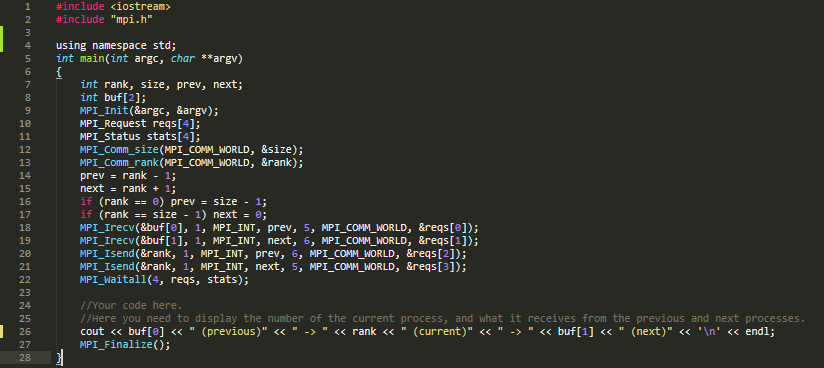
\includegraphics[scale=0.75]{10.code.png}

Assignment 10
\end{center}

The overall goal of the program is that all processes exchange messages with their nearest neighbors (on the left - previous, on the right - next) in accordance with the topology of the ring. Witg \textsc{MPI\_Waitall} the execution of the process is blocked until all exchange operations on the specified \textsc{reqs} identifiers (lines 18-21) are completed and if the error exists in this operations, then the error field in the \textsc{stats} array elements will be set to the appropriate value. In lines $18-21$ there are operations \textsc{MPI\_Irecv} and \textsc{MPI\_Isend} which are equal to previous functions \textsc{MPI\_Recv} and \textsc{MPI\_Send} but in this functions the return from the function occurs immediately after the initialization of the receiving/transmitting process without waiting for the receipt/ processing of the entire message, so we can solve the problem with blocking operations in \textsc{MPI\_Send} and \textsc{MPI\_Recv}. In this lines the process waiting for their neareset neighbours and save information in int array \textsc{buf} and send information about yourself's rank to previous and next. The result is displayed on screens - ring topology works.

\newpage
\subsection{Assignment 11.MPI. Combined reception and transmission of messages.}

\subsubsection{Formulation of the problem}

Based on \textsc{Assignment 10}, write a program for ring topology exchange using the \textbf{MPI\_Sendrecv()} function.

In situations where you need to exchange data between processes, it is safer to use the overlaid 
\textbf{MPI\_Sendrecv} operation. The \textbf{MPI\_Sendrecv} function combines the execution of the send and receive 
operations. Both operations use the same communicator, but message IDs may differ. The location of the 
received and transmitted data in the address space of the process should not overlap. The data sent can be 
of different types and lengths.

In cases when it is necessary to exchange data of the same type with replacement of the sent data with the 
received ones, it is more convenient to use the \textbf{MPI\_Sendrecv\_replace} function. In this operation, the data 
sent from the buf array is replaced with the received data.

The special address \textbf{MPI\_PROC\_NULL} can be used for source and dest in data transfer operations. 
Communication operations with such an address do nothing. The use of this address is convenient instead of 
using logical constructs to analyze the conditions to send / read a message or not.


int \textbf{MPI\_Sendrecv} (
\begin{itemize}
	\item void *\textbf{sendbuf} - the address of the data to be sent
	\item int \textbf{sendcount} - the number of sent variables
	\item MPI\_Datatype \textbf{sendtype} - the type of data being sent
	\item int \textbf{dest} - destination rank
	\item int \textbf{sendtag} - the tag of the sent message
	\item void *recvbuf
	\item int \textbf{recvcount} - is the number of received data
	\item MPI\_Datatype \textbf{recvtype} - the type of data being received
	\item int \textbf{source} - from whom the message is received
	\item int \textbf{recvtag} - received message tag
	\item MPI\_Comm \textbf{comm} - MPI\_Comm comm
	\item MPI\_Status *\textbf{status} - status

\end{itemize}
)

\subsubsection{Example of launch parameters and output. Detailed description of solution}

Code for \textbf{assignment 11} is \href{https:\//github.com/aptmess/parallel_algorithms/blob/master/HT/hw_mpi/Assignment11.c}{here}.

Compilation example: \textsc{mpic++ -o ./cpf/11.o Assignment11.c}

Launch example: \textsc{mpirun --oversubscribe -np 11 ./cpf/11.o}

\begin{center}
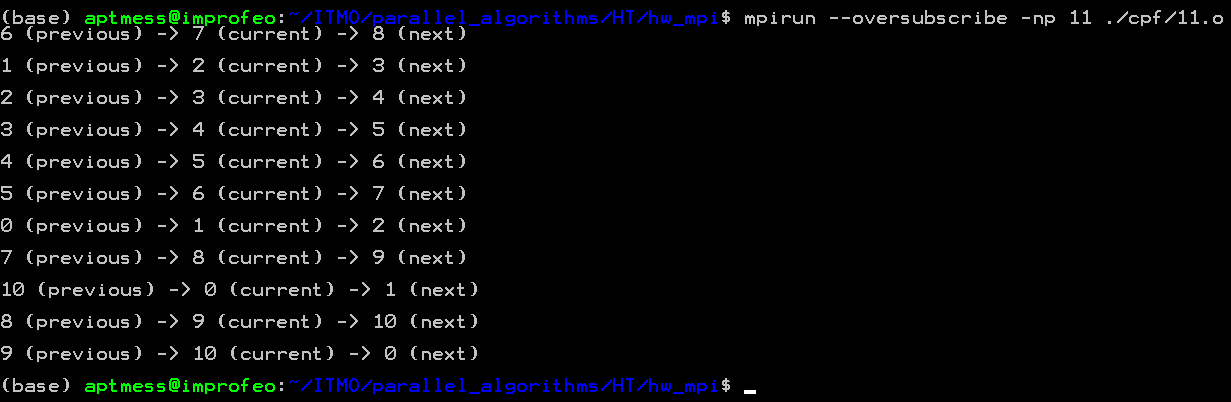
\includegraphics[scale=0.5]{11.png}
\end{center}

Let's move to the the code and explain how it works.

\begin{center}
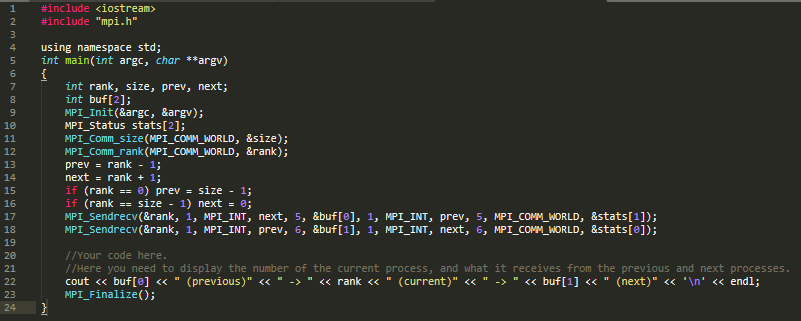
\includegraphics[scale=0.75]{11.code.png}

Assignment 11
\end{center}

The main goal of program is the same as in Assignment 10 and the resuls is equally the same, but in assignment 11 we are using function \textbf{MPI\_Sendrecv()} due to syntax in previous subsection which is sending and try to recieive message in the same function. On line $17$ this function process sends a message with current process's rank to next neareast process and recieve rank of the previous nearest process. On the line $18$ on the contrary - sends a message with rank to previous nearest process and try to recieve rank from nearest next process. The program works correctly.


\subsection{Appendix}

The link to the sourse code which is placed on my \href{https://github.com/aptmess/parallel_algorithms}{github}.


\end{document}